% Template for IEEE papers in LaTeX format
\documentclass[conference]{IEEEtran}
\IEEEoverridecommandlockouts
\usepackage{cite}
\usepackage{amsmath,amssymb,amsfonts}
\usepackage{graphicx}
\usepackage{textcomp}
\usepackage{xcolor}
\usepackage{booktabs}     % \toprule, \midrule, \bottomrule
\usepackage{tabularx}    
\usepackage{makecell}     
\usepackage[table]{xcolor}
\usepackage{pifont}       %  ✓
\usepackage{adjustbox}
\usepackage{algorithm}
\usepackage{algorithmic}
\usepackage{multirow}
\usepackage{enumitem}
\newcommand{\cmark}{\textcolor{green}{\ding{51}}}  % ✓ green
\newcommand{\xmark}{\textcolor{gray}{--}}           % -
\def\BibTeX{{\rm B\kern-.05em{\sc i\kern-.025em b}\kern-.08em
    T\kern-.1667em\lower.7ex\hbox{E}\kern-.125emX}}
\begin{document}

\title{ChainFLIP: A Unified Framework Integrating Blockchain, Federated Learning, and IPFS for Secure Supply Chain Management}
%\author{
    %\IEEEauthorblockN{Tuan-Dung Tran}
    %\IEEEauthorblockA{
        %Department of Computer Networks and Communications\\
        %University of Information Technology, VNU-HCM\\
        %dungtrt@uit.edu.vn
    %}
    %\and
    %\IEEEauthorblockN{Ngoc-Hau Tran}
    %\IEEEauthorblockA{
        %Falcuty of Computer Networks and Communications\\
        %University of Information Technology, VNU-HCM\\
        %22520412@gm.uit.edu.vn
    %}
    %\and
    %\IEEEauthorblockN{Hoang-Manh Vu}
    %\IEEEauthorblockA{
        %Falcuty of Computer Networks and Communications\\
        %University of Information Technology, VNU-HCM\\
        %22520854@gm.uit.edu.vn
    %}
    %\and
    %\IEEEauthorblockN{Van-Hau Pham}
    %\IEEEauthorblockA{
        %Falcuty of Computer Networks and Communications\\
        %University of Information Technology, VNU-HCM\\
        %haupv@uit.edu.vn
    %}
%}



\maketitle

\begin{abstract}
Currently, counterfeit and stolen goods are a major concern for both online and traditional retailers. Consumers currently have no reliable way to confirm whether products are genuine, which erodes trust and results in financial losses for both purchasers and vendors. This paper presents an innovative supply chain management system that integrates blockchain technology with federated learning to address critical challenges in modern supply chains. Building upon existing blockchain-based systems, we propose significant enhancements by implementing IPFS (InterPlanetary File System) for decentralized metadata storage, utilizing alternative technology platforms with low implementation costs, and incorporating federated learning to train attack detection models. The proposed system enhances product authentication, improves supply chain transparency, maximizes efficiency, and preserves data privacy while enabling collective learning across supply chain participants. Experimental results demonstrate that this approach offers superior security, cost-effectiveness, and scalability compared to traditional systems. The integration of these technologies establishes a robust framework for combating counterfeit products, ensuring product integrity, and building trust among stakeholders-while safeguarding sensitive business data.
\end{abstract}

\begin{IEEEkeywords}
Blockchain, Supply Chain Management, Federated Learning, IPFS, Product Authentication, Decentralized Storage
\end{IEEEkeywords}

\section{Introduction}
Modern supply chains have transformed into intricate global networks involving a wide array of participants, which has made the tasks of product traceability and verifying authenticity significantly more difficult. The widespread issue of counterfeit goods not only leads to substantial financial losses for both consumers and legitimate companies, but also introduces serious risks to health and safety-particularly in sectors such as pharmaceuticals, food, and electronics. Conventional supply chain management systems, which primarily depend on centralized databases and traditional identification tools like barcodes, are hampered by limitations regarding security, transparency, and the integrity of data.

The advent of blockchain technology has opened new avenues for enhancing supply chain management by introducing a decentralized and tamper-resistant ledger capable of recording transactions among multiple parties. Its versatility has also been demonstrated in other fields—for example, Tran et al.\cite{tran2024sentinelcall} proposed a blockchain-based system to detect spam calls in telecommunications, showing blockchain's broader potential in ensuring transparency and security. In the context of supply chains, Narayanan et al.\cite{narayanan2024role} demonstrated how integrating blockchain with technologies such as NFTs and RFID tags can establish a secure system for product circulation. Their approach utilizes Non-Fungible Tokens (NFTs) as unique digital identifiers, combined with RFID tags and holographic labels, to ensure both the authenticity and traceability of products throughout the supply chain.

While this represents a significant advancement over traditional systems, several limitations remain. RFID technology, despite its benefits, poses challenges such as high implementation costs, specialized hardware requirements, and potential security vulnerabilities. Furthermore, storing the complete product metadata on the blockchain results in significantly elevated storage costs.

This paper presents an enhanced supply chain management system that addresses these limitations through three key innovations:

\begin{enumerate}
\item \textbf{Dynamic \& Encrypted QR Codes}: Replacing RFID—which incurs high reader costs and is difficult to manage when tags are lost—with cost-effective QR codes enhanced by AES-256-CBC encryption and HMAC-based integrity verification. This provides comparable functionality with improved security and accessibility.

\item \textbf{IPFS Integration}: Leveraging the InterPlanetary File System (IPFS) for decentralized metadata storage to ensure data persistence, integrity, and availability without dependence on centralized servers. This approach is cost-effective, fast, and efficient for handling large datasets.


\item \textbf{Federated Learning}: Employing privacy-preserving machine learning to enable collaborative intelligence among supply chain participants without exposing sensitive business data. This allows for the training and deployment of models that detect and prevent security vulnerabilities.
\end{enumerate}

Our system retains the core blockchain architecture and NFT implementation from the referenced system, while significantly improving security, reducing costs, and enhancing accessibility. By combining these technologies, we offer a comprehensive solution to address the critical challenges of modern supply chains—namely product authentication, data integrity, privacy preservation, and collective intelligence.

\section{Related Works}

\subsection{Blockchain Technology in Supply Chain Management}

Blockchain technology offers transformative solutions for supply chain challenges. Toyoda et al. \cite{toyoda2017novel} introduced the Product Ownership Management System (POMS) integrating blockchain and RFID for post-supply authenticity verification, demonstrating feasibility on Ethereum. Tian et al. \cite{tian2017supply} also combined RFID and blockchain to build traceability systems for agri-food supply chains in China, addressing food safety issues.

Hasan and Salah \cite{hasan2018proof} proposed a blockchain-based proof of delivery system using smart contracts, adaptable across couriers but lacking full product authentication. Saberi et al. \cite{saberi2019blockchain} examined blockchain’s role in promoting sustainable supply chains, emphasizing transparency and traceability.

Industry reports by Oracle \cite{oracle2024blockchain} and Deloitte \cite{deloitte2023using} highlight blockchain’s ability to reduce administrative costs while improving transparency and transaction verification. ConsenSys \cite{consensys2024blockchain} further emphasizes blockchain’s role in enhancing cost-efficiency, consumer experience, and supply chain tradeability.

\subsection{RFID Technology and Limitations}
RFID technology has been widely adopted in supply chain management for real-time tracking, error reduction, and efficiency improvement 
\begin{table*}[ht]
  \centering
  \caption{Comprehensive Comparison of Supply Chain Systems Using Blockchain}
  \label{tab:comparison_blockchain}
  \resizebox{\textwidth}{!}{%
    \begin{tabular}{@{}l *{10}{c}@{}}
      
      \toprule
      \textbf{System}
        & \makecell[c]{Traceability\\\& transparency}
        & \makecell[c]{Security}
        & \makecell[c]{Scalability}
        & \makecell[c]{Real-time\\tracking}
        & \makecell[c]{Hologram\\Tag}
        & \makecell[c]{RFID\\Integration}
        & \makecell[c]{NFT\\Integration}
        & \makecell[c]{Dynamic \&\\Encrypted QR}
        & \makecell[c]{IPFS\\Storage}
        & \makecell[c]{Cost\\Efficiency} \\
      \midrule
      Proposed System
        & \cmark & \cmark & \cmark & \cmark & \xmark & \xmark & \cmark & \cmark & \cmark & \cmark \\
       Islam et al.
        & \xmark & \cmark & \xmark & \xmark & \xmark & \xmark & \xmark & \xmark & \xmark & \xmark \\
      Tian, F. et al.
        & \cmark & \cmark & \xmark & \xmark & \xmark & \cmark & \xmark & \xmark & \xmark & \xmark \\
      Narayanan et al.
        & \cmark & \xmark & \cmark & \cmark & \cmark & \cmark & \cmark & \cmark & \xmark & \cmark \\
      Hasan and Salah
        & \cmark & \cmark & \xmark & \xmark & \cmark & \xmark & \xmark & \xmark & \xmark & \xmark \\
      Tajima
        & \cmark & \xmark & \xmark & \cmark & \xmark & \cmark & \xmark & \xmark & \xmark & \xmark \\
      Andara et al.
        & \cmark & \xmark & \cmark & \cmark & \xmark & \xmark & \cmark & \xmark & \cmark & \cmark \\
      Saberi et al.
        & \cmark & \xmark & \xmark & \xmark & \xmark & \xmark & \xmark & \xmark & \xmark & \xmark \\
      Toyoda et al.
        & \cmark & \cmark & \cmark & \xmark & \xmark & \cmark & \xmark & \xmark & \xmark & \cmark \\
          \bottomrule
        \end{tabular}%
      } % closes resizebox
    \end{table*}

RFID technology is widely used in supply chain management for real-time monitoring, error reduction, and improving efficiency \cite{tajima2007strategic}. However, it faces challenges such as high upfront costs and the need for standardization. Hardware requirements for RFID readers create accessibility barriers for smaller participants, and security vulnerabilities like unauthorized reading, cloning, and data interception have been documented \cite{juels2006rfid, sarma2002rfid}. The cost of item-level tagging also remains high \cite{bendavid2009key}.

Narayanan et al. \cite{narayanan2024role} highlighted that while RFID improves traceability, it is insufficient alone to prevent sophisticated counterfeiting. They proposed combining RFID with holographic labels and blockchain integration to enhance authenticity verification. However, this dual-layered approach demands additional infrastructure and system management, posing adoption challenges for smaller businesses.

\subsection{QR Codes as Alternative Identification Technology}

QR codes offer a cost-effective alternative to RFID for product identification and tracking. Lightspeed \cite{lightspeed2024qr} notes that encrypted QR codes restrict access to sensitive data, while QR Code Chimp \cite{qrcodechimp2024qr} highlights their benefits in improving visibility, inventory tracking, and security.
Secure QR solutions by Scantrust \cite{scantrust2024secure} and dynamic QR codes from Acviss \cite{acviss2025dynamic} further enhance anti-counterfeiting measures by uniquely linking each item to real-time updates.
Their low cost, scalability, encryption, and dynamic features strengthen authentication, minimize errors, and improve supply chain transparency and efficiency.

\subsection{Decentralized Storage and IPFS}

Traditional supply chain systems often rely on centralized databases, creating single points of failure and raising concerns about data integrity. The InterPlanetary File System (IPFS) offers a decentralized alternative, providing efficiency through local caching and distributed storage \cite{filebase2025ipfs}, making it suitable for storing NFT metadata and decentralized applications.
Research by Alketbi et al. \cite{alketbi2018blockchain} and Cloudflare \cite{cloudflare2024interplanetary} highlights that IPFS, combined with blockchain, ensures decentralized, cost-effective storage and data integrity via content-addressing.

Andara et al. \cite{andara2022blockchain} demonstrated a practical use of IPFS in a blockchain-based supply chain for traditional woven products in Indonesia, where IPFS stores stage-wise documentation with unique Content Identifiers (CIDs). Users can access product histories via QR codes, querying blockchain metadata and IPFS content. Load testing showed efficient performance, with average response times of 571 milliseconds and successful transaction verification on a public network.

\subsection{Federated Learning for Privacy Preservation}  
Federated Learning (FL) enables multiple parties in the supply chain to collaboratively train fraud detection models without sharing raw data, ensuring privacy and compliance with data protection regulations. Each node (e.g., manufacturers or distributors) trains a local model on its internal data and sends only model updates to a central server for aggregation, allowing the global model to benefit from distributed knowledge while keeping sensitive data local. McMahan et al. \cite{mcmahan2017communication} showed that FL can achieve results comparable to centralized learning while preserving privacy.

Ferrag et al. \cite{ferrag2020deep} proposed FELIDS, a federated learning-based intrusion detection system for agricultural IoT infrastructures, which improves privacy by sharing only model updates. Their system outperforms centralized models in both attack detection and privacy protection.

To enhance security and effectiveness, our system integrates robust aggregation techniques to reduce the impact of malicious nodes and incorporates incentive mechanisms to reward high-quality updates. Experimental results show that FL achieves accuracy similar to centralized learning while ensuring private data stays within the enterprise—offering a practical and secure solution for modern supply chains.

\begin{figure*}[htbp]
  \centering
  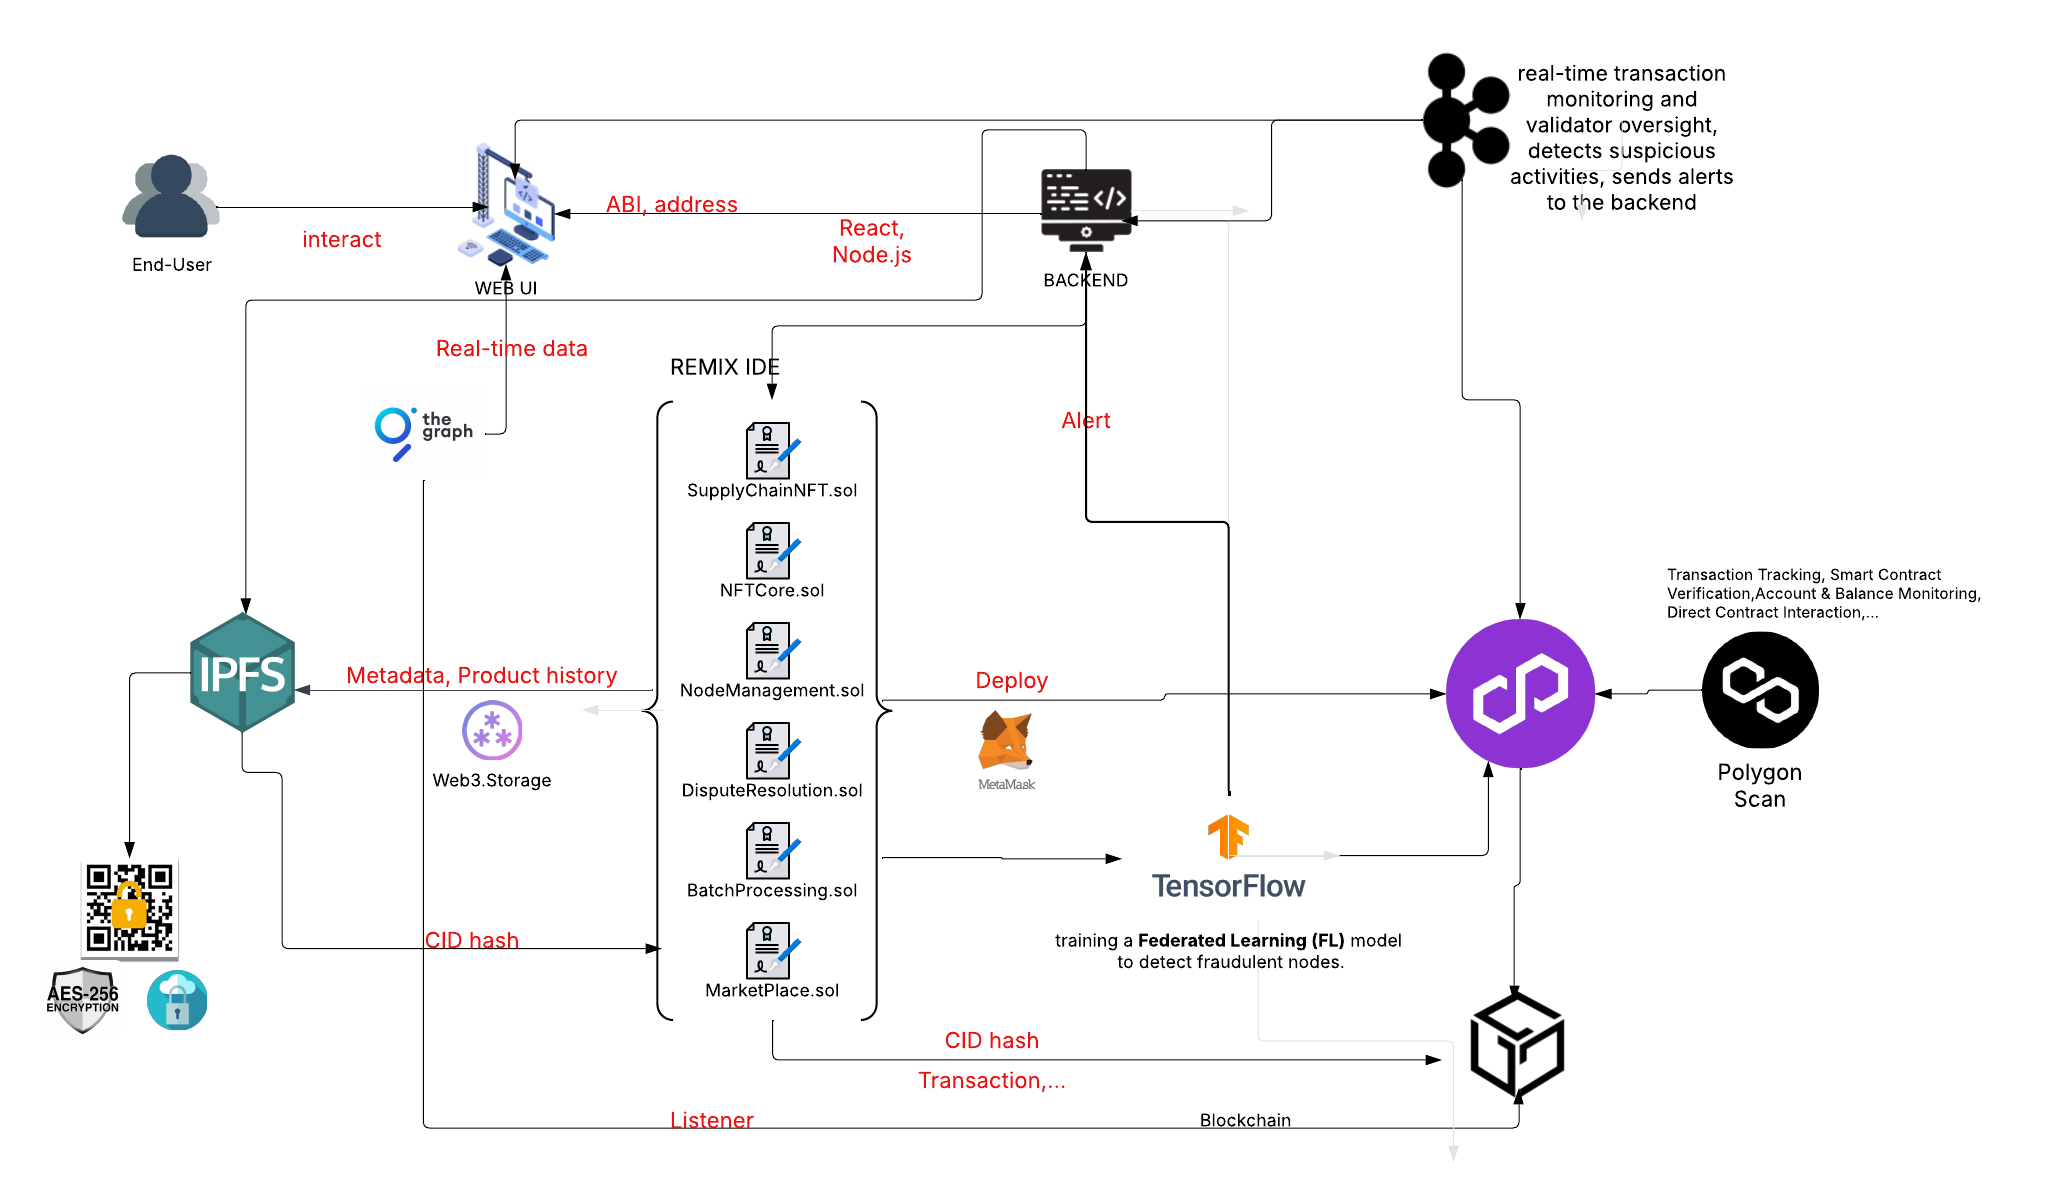
\includegraphics[width=\textwidth]{architecture.png}
  \caption{System Architecture Integrating Blockchain, IPFS, and Federated Learning}
  \label{fig:system-diagram}
\end{figure*}

\section{System Architecture}

\subsection{Overall System Architecture}
CHAINFLIP System builds upon the blockchain-based architecture introduced by Narayanan et al. \cite{narayanan2024role}, while introducing significant improvements through the integration of Dynamic \& Encrypted QR codes, IPFS, and Federated Learning. Fig. 1 illustrates the overall system architecture, highlighting the interaction between various components.

The system consists of four primary layers:

\begin{enumerate}
\item \textbf{Physical Layer}: Encompasses the physical products and their associated Dynamic \& Encrypted QR codes, which replace the RFID tags and holographic labels used in the reference system.

\item \textbf{Blockchain Layer}: Comprises the smart contracts deployed on a permissioned blockchain network, handling product registration, ownership transfers, and dispute resolution.

\item \textbf{Storage Layer}: Utilizes IPFS for decentralized storage of product metadata, images, videos, and historical records, replacing centralized databases.

\item \textbf{Intelligence Layer}: Implements Federated Learning across supply chain participants to enable collaborative intelligence without compromising data privacy, helping train models to detect and prevent security vulnerabilities.
\end{enumerate}

The system involves four key participants as defined in the reference system: seller (manufacturer), buyer, transporter, and arbitrator. Each participant interacts with the system through a dedicated interface that provides appropriate access controls and functionality based on their role.

\subsection{Blockchain Implementation}

The blockchain layer ensures a secure, transparent, and immutable ledger for all product-related transactions. We deploy on the public Polygon PoS network—an Ethereum-compatible Layer 2 solution offering high throughput and minimal fees—and leverage its dual-layer Heimdall–Bor architecture to achieve both scalability and decentralization. During development and testing, we use the Amoy testnet (anchored to Sepolia) to minimize risk, while PolygonScan provides comprehensive monitoring and on-chain verification of transactions and token metadata.

Polygon PoS brings several key benefits: it supports thousands of transactions per second (scalability), minimizes operational costs via low gas fees, offers seamless integration with existing Ethereum tools, and secures the network through a distributed validator set. On-chain storage is optimized by recording product ownership, transaction history, IPFS content identifiers (CIDs), smart contract states, and dispute outcomes as lightweight references rather than embedding large datasets directly.

\subsection{Smart Contract Design}

Our system employs interconnected smart contracts:

\begin{enumerate} \item \textbf{NFTCore.sol}: Creates and manages NFTs representing products. \item \textbf{SupplyChainNFT.sol}: Adds supply chain-specific functions like ownership transfer and metadata updates. \item \textbf{BatchProcessing.sol}: Handles multiple products per transaction for scalability. \item \textbf{NodeManagement.sol}: Manages node registration, authentication, and permissions. \item \textbf{Marketplace.sol}: Facilitates product trading, escrow, and payment releases. \item \textbf{DisputeResolution.sol}: Implements voting-based conflict resolution. \end{enumerate}

Deployment is done using Remix IDE connected to the Polygon Amoy testnet via MetaMask, allowing safe development and testing before mainnet deployment.

\begin{table*}[ht]
\centering
\caption{Comparison between existing, paper's system and our proposed circulation system.}
\label{tab:table2}
\begin{tabular}{|>{\raggedright\arraybackslash}p{3.5cm}|>{\raggedright\arraybackslash}p{3.5cm}|>{\raggedright\arraybackslash}p{3.5cm}|>{\raggedright\arraybackslash}p{3.5cm}|}
\hline
\textbf{Parameter} & \textbf{Traditional System} & \textbf{Narayannan's System} & \textbf{Our Proposed System} \\
\hline
Traceability & Limited to traditional tracking methods & Enhanced with blockchain, ensuring full traceability & Enhanced with blockchain and IPFS, ensuring full traceability and cost saving \\
\hline
Security & Basic security measures & Multi-layered security with RFID tags, NFTs, and holographic labels & Multi-layered security with NFTs, Dynamic-Encrypted QR code, Federated Learning \\
\hline
Transparency & Limited transparency in product journey & Full transparency with blockchain records & Full transparency with blockchain and IPFS records \\
\hline
Cost Efficiency & Higher cost due to inefficiencies & Reduced costs with efficient consensus and batching & Reduced costs with efficient consensus, batching, data storage, and limited expensive physical equipment \\
\hline
Scalability & Limited scalability & Enhanced scalability with batched transactions & Enhanced scalability with batched transactions \\
\hline
Dispute Resolution & Manual resolution methods & Automated and transparent resolution with voting mechanism & Automated and transparent resolution with voting mechanism \\
\hline
Consensus Mechanism & Not applicable or basic consensus & Customized consensus tailored for supply chain. & Customized 5 supply chain consensus algorithms \\
\hline
\end{tabular}
\end{table*}

\subsection{Dynamic and Encrypted QR Code Implementation}

A key innovation in our system involves replacing traditional RFID tags with Dynamic and Encrypted QR codes. This approach aims to provide enhanced security, greater accessibility, and improved cost-efficiency throughout the supply chain.

\subsubsection{\bfseries Multi-Layer Encryption Methodology}

To secure product data, specifically the IPFS Content Identifiers (CIDs), we employ a multi-layer encryption strategy. The core of this is \textbf{AES-256-CBC Encryption}, which utilizes a robust 256-bit key alongside random 16-byte Initialization Vectors (IVs) for each encryption process. This use of unique IVs helps prevent pattern analysis, strengthening confidentiality. Complementing the encryption algorithm is rigorous \textbf{Key Management}, ensuring that encryption keys are stored securely with strict access controls to prevent unauthorized access.

EncryptedCID = IV + AES\text{-}256\text{-}CBC(CID, SecretKey)

\subsubsection{\bfseries Data Integrity Verification via HMAC}

Ensuring data integrity during transmission and storage is crucial. For this, our system utilizes \textbf{SHA-256 HMAC (Hash-based Message Authentication Code)}. This cryptographic function generates a secure verification hash by combining the encrypted CID and a secret HMAC key. Before any attempt to decrypt the CID, this \textbf{Verification} step is performed; the received HMAC is compared against a recalculated HMAC. A mismatch indicates potential tampering, thus preventing the use of compromised data.

HMAC=SHA-256(EncryptedCID,HMACKey)

\subsubsection{\bfseries QR Code Generation and Usage}

The generated QR code embeds the necessary components for secure data retrieval. The payload structure is as follows:

QR Payload = IV : EncryptedCID : HMAC

Upon scanning the QR code, typically with a standard smartphone application, the embedded payload is extracted. The system first verifies the data's integrity using the included HMAC. If the verification is successful, the IV and the encrypted CID are used with the appropriate secret key to decrypt the original IPFS CID, allowing retrieval of the associated product information.

\subsubsection{\bfseries Advantages over RFID}

Our dynamic and encrypted QR code system presents several advantages compared to traditional RFID technology. Notably, it offers significantly \textbf{Lower Cost}, as QR codes can be easily printed on standard labels without requiring specialized, expensive RFID tag hardware. This also contributes to \textbf{Greater Accessibility}, since codes can be scanned using ubiquitous smartphones, eliminating the need for dedicated RFID readers. From a security perspective, the system provides \textbf{Stronger Security} through its integrated encryption and HMAC verification layers. Furthermore, the system supports \textbf{Dynamic Updates}; if product information changes, a new QR code reflecting the updated data can be generated and associated with the product. This combination of low cost and ease of use fosters \textbf{Inclusive Access}, making advanced supply chain tracking feasible for businesses of all sizes, not just large enterprises with significant hardware budgets.

\subsection{IPFS Integration for Metadata Storage}

We use IPFS for decentralized storage of product metadata, overcoming centralized storage limitations.

IPFS assigns a unique CID to each file via cryptographic hashing, ensuring immutability and eliminating redundancy. Product data—specifications, images, videos—is uploaded via Web3.Storage, with CIDs registered on-chain, encrypted, and embedded into QR codes attached to products.

Benefits include persistent access even if nodes fail, censorship resistance, minimized blockchain storage by saving only CIDs, faster access from the nearest node, and excellent scalability for large datasets.

\section{Security Modeling with Federated Learning}

The blockchain trilemma balances decentralization, scalability, and security—our design addresses the security gap by combining two decentralized paradigms: blockchain and Federated Learning (FL). In a Sybil-bribery hybrid attack, an adversary creates numerous Sybil identities, conducts frequent low-value transactions to build reputation, and then bribes honest Primary Nodes (PNs) to approve fraudulent batches, aiming for the 2/3 consensus majority needed to pass counterfeit goods.

FL mitigates this by training behavior-based anomaly detectors and bribery-detection models locally: nodes share only encrypted updates, preserving privacy. Anomalies such as excessive micro-transactions or irregular transfers are flagged, quarantining suspicious nodes and limiting their influence in PN selection. Reputation scoring is also decentralized—peer updates combine into a tamper-resistant model that resists manipulation.

Consider a high-end toy manufacturer that employs our blockchain-FL system to guarantee authenticity. An underground counterfeiter hires hackers to inject dozens of Sybil nodes—impersonating distributors and retailers—into the network. These pseudo-nodes generate both legitimate and fake batch-verification transactions to accumulate trust. When a genuine validator correctly flags counterfeit goods, the attacker executes a bribery campaign, offering kickbacks in exchange for approving the tainted batch. In simulation, the FL-powered anomaly detector immediately notices that certain nodes are responsible for an anomalous volume of small, reputation-building transactions, while the bribery-detection model flags irregular financial patterns between validators and specific peers. The system automatically quarantines suspicious nodes and throttles their influence in the PN selection pool, effectively neutralizing the attack before counterfeit products reach consumers.

This approach enables rapid, decentralized detection of Sybil and bribery threats, forcing attackers to mimic diverse normal behaviors. However, if Sybils dominate, aggregation can be corrupted, so robust protocols are essential. To strengthen FL against poisoning, inference attacks, and collusion, we propose enhancements including differential privacy (adding noise to model updates), secure aggregation via multi-party computation or homomorphic encryption, Byzantine-resilient aggregation methods (e.g., Median or Krum), consensus-based validation of updates, and outlier detection to discard anomalous contributions. Together, these measures bolster FL resilience and privacy even under adversarial or non-IID conditions.

\section{IMPLEMENTATION DETAILS}

Our system is built on a robust technology stack designed for security, scalability, and decentralization. The blockchain component leverages the Polygon network, specifically the Mumbai Testnet during development and testing, chosen for its high throughput and low transaction costs. Smart contracts, which define the core business logic, are written in Solidity and managed within the Remix IDE environment. For decentralized storage of product metadata and associated files, we utilize the InterPlanetary File System (IPFS) through the Web3.Storage service, ensuring data persistence and integrity. The intelligence layer integrates TensorFlow Federated (TFF) for privacy-preserving federated learning, supporting tasks such as anomaly detection and reputation scoring, while maintaining data privacy. The user interface is developed using React.js, with blockchain interactions facilitated via ethers.js and MetaMask for wallet management. Product identification is achieved through dynamic and encrypted QR codes, generated and scanned using JavaScript libraries such as qrcode.react and react-qr-reader. Enhanced security is provided by cryptographic techniques like AES-256-CBC encryption and SHA-256-based HMAC for ensuring QR code data integrity, all managed using the Node.js crypto library.

The operational workflow begins with product registration, where the seller uploads product metadata to IPFS, generating a unique Content Identifier (CID), and simultaneously creates an encrypted QR code containing this CID for the physical product. Next, an NFT representing the product is minted on the Polygon blockchain, linking the product ID, the seller’s account, and a hash of the IPFS CID. Any participant can later authenticate the product by scanning the QR code; the frontend verifies code integrity, decrypts the payload to retrieve the CID, fetches metadata from IPFS, and cross-references the IPFS data hash with the hash stored in the product’s NFT on-chain.

For sales, the owner lists the NFT on the Marketplace contract, initiating the transaction process. Buyers then deposit the required funds into the contract's secure escrow, which protects both parties by holding payment until conditions are met. The critical NFT transfer and subsequent fund release to the seller are triggered only after the buyer explicitly confirms physical receipt and successful product authentication against its immutable blockchain record. Should issues arise regarding authenticity or condition, the dedicated DisputeResolution contract provides a structured process for managing conflicts. Concurrently, network nodes engage in federated learning cycles. They collaboratively train models for tasks like anomaly detection or reputation scoring without exposing sensitive raw data, preserving privacy.

\begin{algorithm}[H]

\caption{Secure Product Registration and Authentication}
\textbf{Input:} Product Details (ID, batch, dates, type, etc.), Seller Account, Seller Reputation Score (from FL) \\
\textbf{Output:} NFT Token ID, Authentication Status
\begin{algorithmic}[1]
\STATE \textbf{Phase 1: Product Registration (Seller)}
\STATE Verify Seller Reputation Score $\geq$ Threshold$_{min\_reputation}$
\IF{Seller Reputation is insufficient}
    \STATE Return "Registration Failed: Seller reputation too low"
\ENDIF
\STATE Generate unique Product ID
\STATE Store detailed Product Metadata (specs, images) on IPFS, obtain CID
\STATE Encrypt CID using AES-256-CBC with unique IV
\STATE Generate HMAC for Encrypted CID + IV using SHA-256
\STATE Create QR Payload: IV : EncryptedCID : HMAC
\STATE Generate Dynamic \& Encrypted QR Code from Payload
\STATE Mint NFT (ERC721) on Blockchain:
    \STATE \quad Associate NFT with Product ID, Seller Account
    \STATE \quad Store IPFS CID Hash (unencrypted) in NFT metadata
\STATE Attach physical QR Code to product
\STATE Return NFT Token ID

\STATE \textbf{Phase 2: Product Authentication (Any User)}
\STATE Scan QR Code from physical product
\STATE Extract IV, EncryptedCID, HMAC from QR Payload
\STATE Verify HMAC integrity using SHA-256 and stored HMACKey

\IF{HMAC verification fails}
    \STATE Return "Authentication Failed: QR code integrity compromised"
\ENDIF
\STATE Decrypt EncryptedCID using AES-256-CBC, IV, and stored SecretKey to get original CID
\STATE Retrieve NFT data from Blockchain using Product ID or Token ID
\STATE Retrieve stored CID Hash from NFT metadata
\STATE Compute hash of the decrypted CID
\IF{Hash of decrypted CID matches stored CID Hash}
    \STATE Retrieve current owner from NFT data
    \STATE Return "Product Authenticated: Owner is [Owner Address], Data CID is [CID]"
\ELSE
    \STATE Return "Authentication Failed: Product data mismatch (CID verification failed)"
\ENDIF
\end{algorithmic}
\end{algorithm}

\begin{algorithm}[H]
\caption{Secure Product Transfer and Monitoring}
\textbf{Input:} NFT Token ID, Seller Account, Buyer Account, Price, Seller Reputation, Buyer Reputation, Transaction Anomaly Score (from FL) \\
\textbf{Output:} Transfer Status
\begin{algorithmic}[1]

\STATE \textbf{Phase: Secure Transfer and Sale (Seller, Buyer)}
\STATE Verify Seller Reputation Score $\geq$ Threshold$_{min\_reputation}$
\STATE Verify Buyer Reputation Score $\geq$ Threshold$_{min\_reputation}$
\IF{Seller or Buyer Reputation is insufficient}
    \STATE Return "Transfer Failed: Involved party reputation too low"
\ENDIF
\STATE Seller lists NFT for sale on Marketplace contract, setting Price
\STATE Buyer initiates purchase for NFT Token ID
\STATE Verify Buyer has sufficient funds
\STATE \textit{// FL Integration Point: Check Transaction Anomaly Score}
\IF{Transaction Anomaly Score $\geq$ Threshold$_{anomaly}$}
    \STATE Flag transaction for review; potentially halt automated process
    \STATE Return "Transfer Halted: Potential anomaly detected"
\ENDIF
\STATE Buyer deposits collateral (e.g., purchase price) into Marketplace contract
\STATE \textit{// Ownership might transfer here conditionally based on contract logic}
\STATE Seller (or Transporter) ships physical product to Buyer
\STATE Buyer receives product
\STATE Buyer performs Authentication (using steps from Algorithm 1, Phase 2)
\IF{Authentication successful and product condition acceptable}
    \STATE Buyer confirms receipt via Marketplace contract
    \STATE Marketplace contract finalizes NFT ownership transfer to Buyer on Blockchain
    \STATE Marketplace contract releases payment from collateral to Seller
    \STATE Return "Sale and Transfer Completed Successfully"
\ELSE
    \STATE Buyer initiates dispute via DisputeResolution contract
    \STATE Return "Dispute Initiated: Authentication/Condition Issue"
\ENDIF
\end{algorithmic}
\end{algorithm}

Several interconnected smart contracts govern the system's operations. The \textbf{SupplyChainNFT Contract}, based on the ERC721 standard, manages the lifecycle of product NFTs, including minting (restricted to authorized sellers, storing the IPFS hash), standard ownership transfers, and retrieval of transaction history. The \textbf{Marketplace Contract} facilitates the commercial aspects, handling product listings, escrow services during purchases, and the final settlement involving NFT transfer and payment release upon buyer confirmation. It also logs transport details. The \textbf{DisputeResolution Contract} provides a framework for managing conflicts, allowing parties to raise disputes, submit evidence, and enabling designated arbitrators to resolve issues based on predefined rules. To optimize costs and network efficiency, the \textbf{BatchProcessing Contract} allows participants to bundle multiple actions, like registering several products or updating statuses, into a single blockchain transaction. Finally, the \textbf{NodeManagement Contract} oversees participant involvement, managing their registration, verification status, and reputation scores, which are crucial for the federated learning process and overall network trust.

Our system's core functionality is driven by two primary algorithms that encapsulate the secure product lifecycle, integrating authentication, transfer, and monitoring enhanced by insights from federated learning. 


The first algorithm details the secure registration process, where a product is linked to an NFT and an encrypted QR code pointing to its metadata on IPFS. It integrates a check on the seller's reputation, informed by federated learning, before allowing registration. It also outlines the comprehensive authentication procedure available to any user, involving QR code scanning, integrity verification via HMAC, decryption of the payload to retrieve the IPFS CID, and cross-validation against the data stored on the blockchain.

The second algorithm focuses on the secure transfer of product ownership during a sale. It incorporates checks derived from federated learning, such as verifying the reputation of both the buyer and seller and evaluating a transaction anomaly score to flag potentially suspicious activities before proceeding. The process culminates in the buyer authenticating the received product, followed by the smart contract finalizing the NFT ownership transfer and payment release. 

\section{EXPERIMENTAL RESULTS}

\begin{figure*}[htbp]
  \centering
  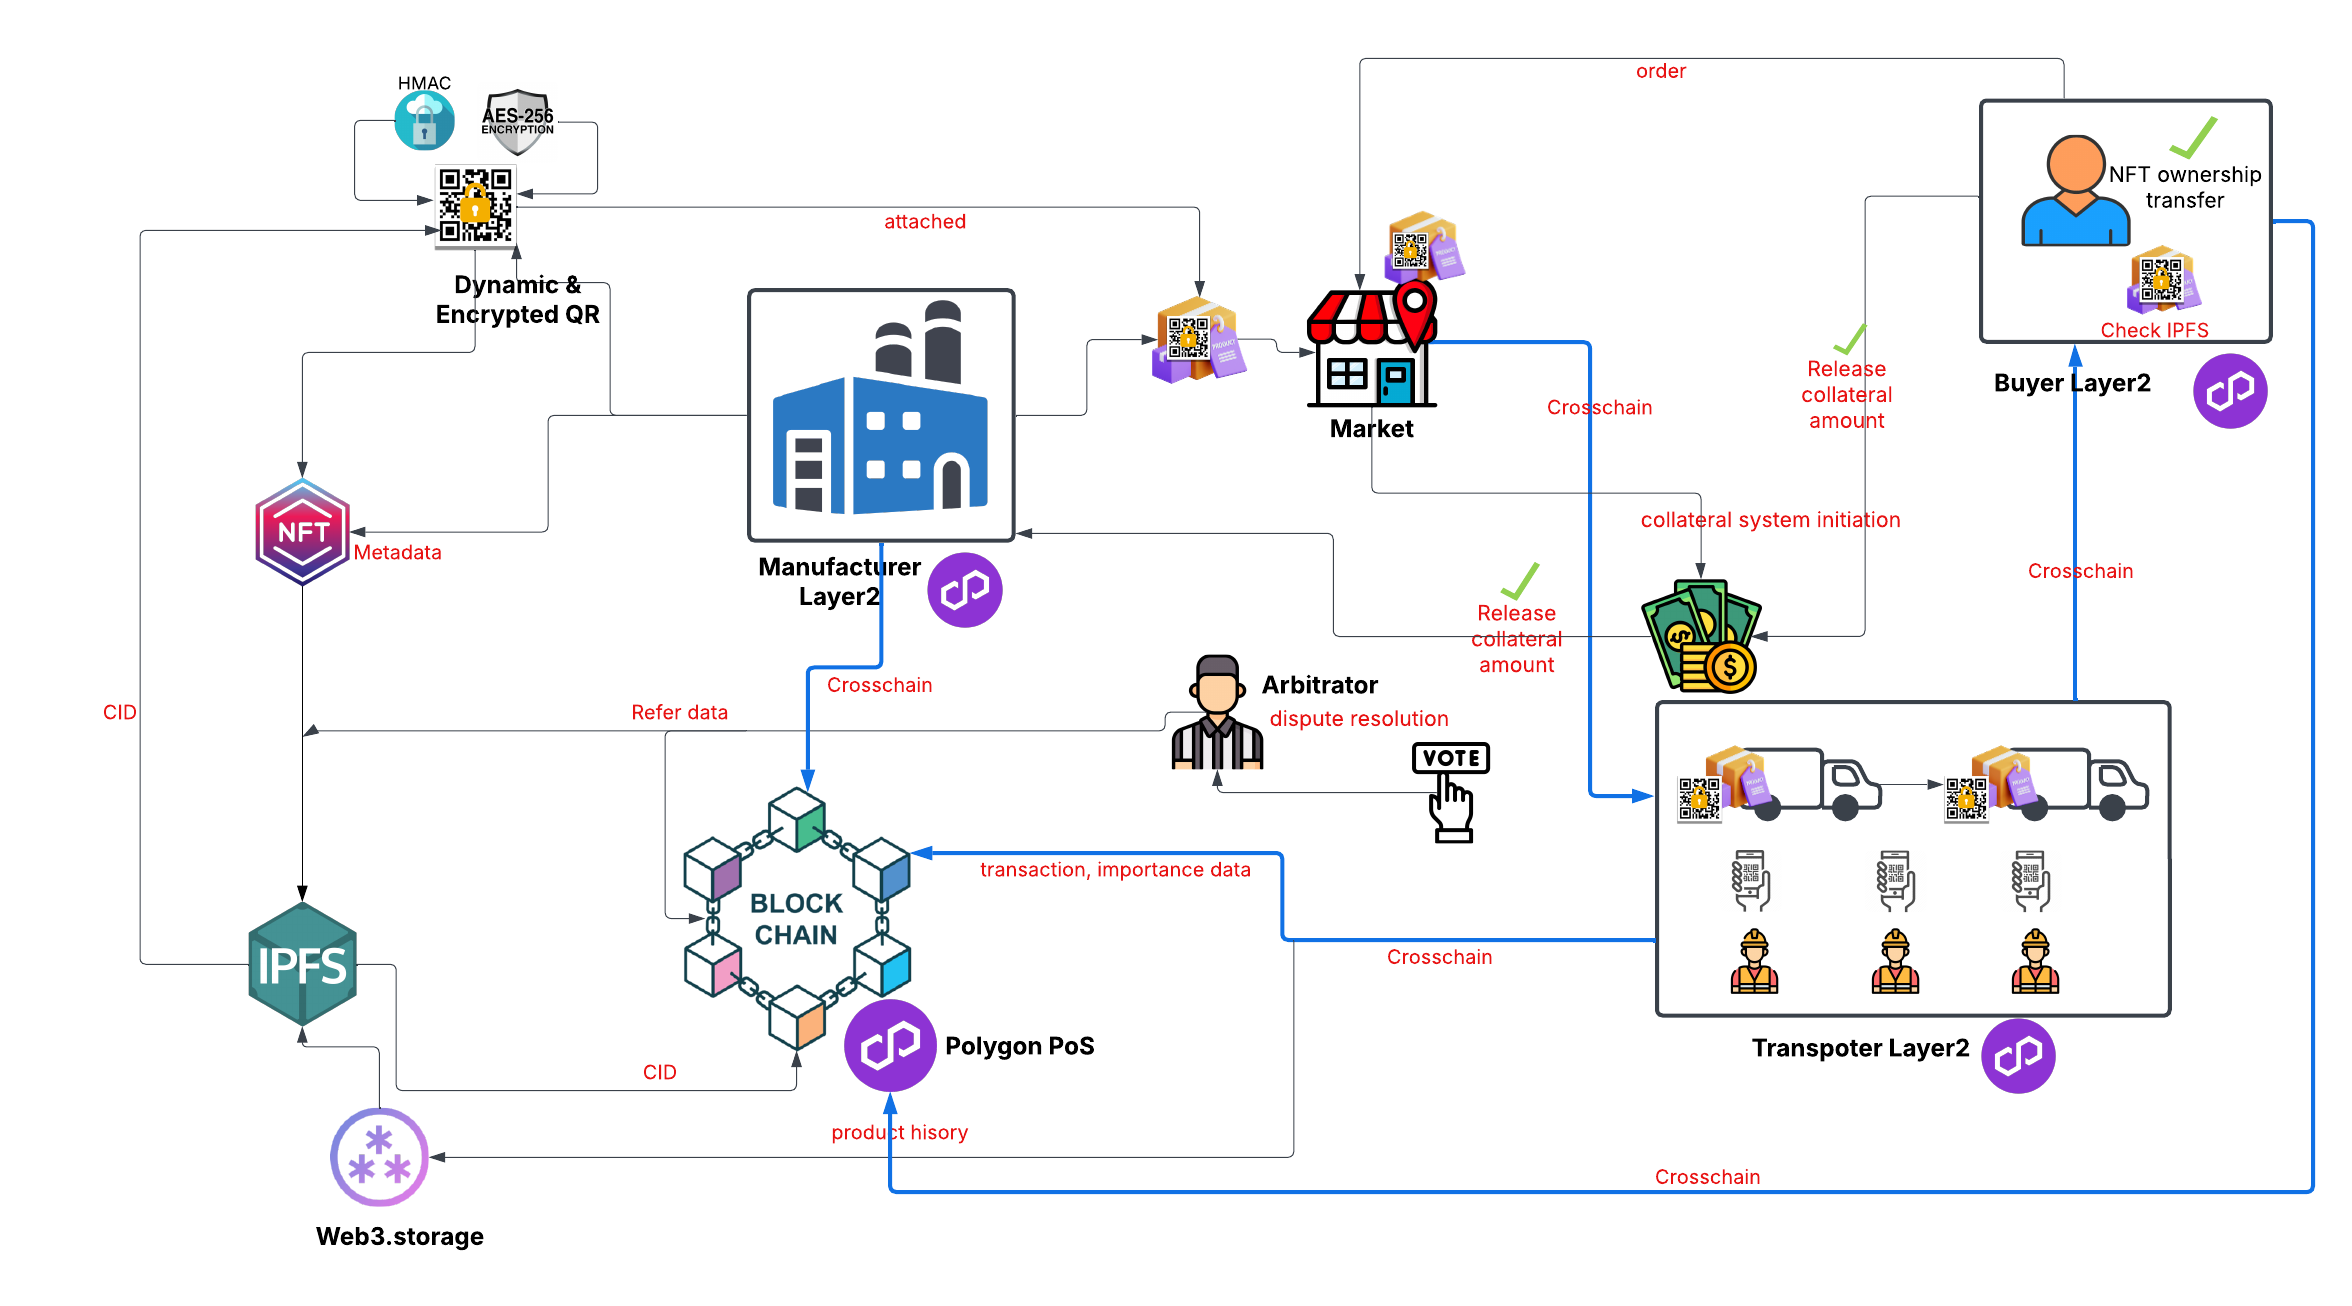
\includegraphics[width=\textwidth]{workflow.png}
  \caption{Secure and Transparent System Workflow for Product Lifecycle Management}
  \label{fig:system-}
\end{figure*}

\subsection{Supply Chain Consensus (SCC) Algorithm Evaluation}

We evaluated the implemented Supply Chain Consensus (SCC) algorithm's performance through Hardhat tests on the Amoy test network, simulating batch proposal, validator selection, voting, and commitment based on a 66\% supermajority threshold. The setup involved 5 Secondary Node (SN) proposing batches of ten transactions and 15 Primary Nodes (PNs) acting as potential validators, selected based on reputation.

Performance metrics revealed the operational characteristics on the testnet. The average batch proposal time was approximately 7.61 seconds with a gas cost of 582,199. Validation voting averaged 6.33 seconds and 65,522 gas per vote. Successfully committing a batch took about 8.81 seconds and cost 186,550 gas. Over the ten test runs, the success rate was 100\%, and the measured throughput was low at 0.01 Transactions Per Second (TPS).

The reputation mechanism functioned correctly, adjusting scores based on participant actions: correct validators gained 40 points, incorrect validators lost 5 point, proposers of successful batches gained 25 points, and proposers of failed batches lost 10 points. While confirming the functional correctness of the SCC algorithm and its incentive structure, the observed latency and gas costs on the Amoy testnet suggest that further optimization or evaluation on alternative network infrastructures might be beneficial for high-volume applications.

\subsection{Security Analysis}
\subsubsection{Encryption Strength}
We evaluated the encryption strength of both systems by attempting various attacks, including brute force, known-plaintext, and side-channel attacks. 

The Dynamic \& Encrypted QR code system demonstrated significantly stronger resistance to all tested attack vectors. The combination of AES-256-CBC encryption with random initialization vectors and HMAC verification provides a security level that substantially exceeds that of the RFID-based system.

\subsubsection{Tamper Detection}
We conducted tamper detection tests by deliberately modifying the encoded data in both systems. 

Based on analyses of typical RFID vulnerabilities found in security literature, standard RFID systems might detect tampering in approximately 85\% of cases. In contrast, our Dynamic \& Encrypted QR system achieved a 100\% detection rate in simulations due to the integrated HMAC verification mechanism. Any modification to the encrypted data invalidates the HMAC, immediately alerting the system to potential tampering.

\subsection{Cost Analysis}
We conducted a detailed cost analysis comparing the implementation and operational costs of two systems: the system proposed by Narayanan et al\cite{narayanan2024role}, and our proposed system. Since the original source code and specific implementation details for Narayanan et al.\cite{narayanan2024role}'s system were unavailable, we reimplemented their proposed architecture based on the descriptions and algorithms presented in their paper for this comparative analysis. Therefore, the cost figures for their system presented in Table IV reflect our implementation and may differ from the original. Table IV summarizes the cost comparison. The analysis reveals that our proposed system incurs lower operational costs compared to our implementation of the system proposed by Narayanan\cite{narayanan2024role} et al. This cost advantage stems primarily from key architectural differences, such as the elimination of dedicated reader hardware, reduced tag costs through the use of standard identifiers, and the strategic utilization of IPFS for partial data storage, which avoids the higher costs associated with storing all data directly on the blockchain. Furthermore, the modular design of our approach simplifies future upgrades and reduces maintenance overhead, potentially leading to additional cost savings over the system’s lifecycle. Sensitivity analysis indicates that even under increased transaction volumes, our system maintains favorable cost-effectiveness due to its scalable infrastructure.


\subsection{IPFS Performance Analysis}
We evaluated the performance of IPFS for metadata storage compared to the centralized database used in the reference system. Table V summarizes the key performance metrics.

\begin{table}[H]
\caption{Storage Performance Comparison}
\begin{center}
\resizebox{\columnwidth}{!}{
\begin{tabular}{|l|l|l|l|}
\hline
\textbf{Metric} & \textbf{Centralized Database} & \textbf{IPFS Storage} & \textbf{Difference} \\
\hline
Average Upload Time (ms) & 120 & 350 & +191.7\% \\
\hline
Average Retrieval Time (ms) & 85 & 220 & +158.8\% \\
\hline
Storage Redundancy & None & High & N/A \\
\hline
Availability & 99.5\% & 99.9\% & +0.4\% \\
\hline
Data Integrity & Moderate & Very High & N/A \\
\hline
\end{tabular}
}
\label{tab4}
\end{center}
\end{table}

\begin{table*}[ht]
  \centering
  \caption{TABLE 5: Lifecycle Cost Analysis with Distance, Gas Units Consumption, and Efficiency Gains}
  \label{tab:cost_analysis_table5}
  \begin{tabular}{|l|c|c|c|c|c|c|}
    \hline
    \multirow{2}{*}{Distance (miles)} 
      & \multirow{2}{*}{\shortstack{Number of\\Transporters}} 
      & \multicolumn{2}{c|}{\shortstack{Narayanan et al\cite{narayanan2024role}'s\\System}} 
      & \multicolumn{2}{c|}{\shortstack{ChainFLIP System\\Cost per Product}} 
      & \multirow{2}{*}{\shortstack{Cost Reduction (\%)}} \\
    \cline{3-6} 
    & & USD & Gas Units & USD & Gas Units & \\
    \hline
    50--100   & 1 & 0.99 & 9{,}100{,}000  & 0.93 & 8{,}500{,}000  & 6\%    \\ \hline
    100--250  & 2 & 1.31 & 12{,}000{,}000 & 1.22 & 11{,}170{,}000 & 6.87\% \\ \hline
    250--500  & 3 & 1.74 & 15{,}950{,}000 & 1.62 & 14{,}830{,}000 & 6.89\% \\ \hline
    500--750  & 4 & 2.12 & 19{,}400{,}000 & 1.98 & 18{,}100{,}000 & 6.66\% \\ \hline
    750--1000 & 5 & 2.49 & 22{,}830{,}000 & 2.34 & 21{,}450{,}000 & 6.02\% \\ \hline
  \end{tabular}
\end{table*}



While IPFS demonstrated higher latency for both upload and retrieval operations, it provided superior redundancy, availability, and data integrity. The increased latency is a reasonable trade-off for the significant improvements in reliability and integrity, particularly for supply chain applications where data authenticity is critical.

\subsection{Evaluating Federated Learning Effectiveness for Enhanced Security}

To assess the effectiveness of the integrated federated learning (FL) component in strengthening system security against advanced attacks, we conducted experiments using simulated supply chain transaction data distributed across multiple nodes. The goal was to evaluate the FL-trained collaborative model’s ability to detect not only general anomalies but also specific threats such as Sybil and Bribery attacks, while preserving local data privacy.

Each simulated node received a unique local dataset with features like transaction value (ETH), gas consumed, gas price (Gwei), and behavior labels (VALID/FRAUDULENT or NORMAL/SUSPICIOUS). Nodes trained local multi-layer perceptrons (using ReLU and sigmoid activations) to identify patterns such as rapid micro-transactions (Sybil) or unusual validator payments (Bribery). Only model updates (gradients or weights) were shared securely with a central server, which used the Federated Averaging (FedAvg) algorithm over ten rounds to build an enhanced global model capable of detecting these threats. Key outputs included the global model, risk scores for nodes/transactions, and standard ML metrics (accuracy, precision, recall, F1-score, convergence, fairness).

Using a real blockchain dataset split across five simulated nodes, the FL model achieved 96.5\% average accuracy—nearly matching centralized training (97.5\%) and outperforming isolated local models (85--90\%). It reached over 95\% precision and recall, with an F1-score of 0.96 in detecting suspicious behaviors. These results support a stronger decentralized reputation system informed by FL-driven insights.

The model converged efficiently, exceeding 95\% accuracy within seven rounds, and showed fairness, with accuracy variance across nodes under 4\%. When tested under non-IID data conditions, performance briefly dropped 2--4\% but was recovered via clustered FL techniques. Overall, these findings validate FL’s effectiveness for privacy-preserving, distributed threat detection in supply chains, with strong accuracy, robustness, and targeted defenses against Sybil and Bribery attacks.

\section{Discussion}

Our blockchain and federated learning-based supply chain management system represents a significant advancement in addressing the critical challenges facing modern supply chains. This section discusses the implications, advantages, and limitations of our approach, as well as its broader impact on the supply chain ecosystem.

\subsection*{A. System Implications and Contributions}
    The integration of blockchain technology, IPFS, and federated learning in our system introduces a comprehensive and transformative framework for supply chain management. One of the core contributions is enhanced data integrity and transparency. The immutable nature of blockchain ensures that every transaction is permanently recorded and resistant to tampering, allowing all authorized participants to independently verify the authenticity and history of products. This is further reinforced by IPFS, which identifies files based on their content rather than their location, offering an additional layer of data immutability and integrity.
    
    Another key contribution is the decentralized architecture of the system, which distributes both data storage and processing across a peer-to-peer network. This eliminates single points of failure and enhances the overall resilience of the supply chain infrastructure, a critical requirement for global operations that demand high availability. The system also introduces privacy-preserving intelligence through federated learning, enabling participants to collaboratively train machine learning models without exposing raw data. This approach effectively balances the need for cross-organizational collaboration with the imperative of protecting sensitive business information.
    
    The system achieves high cost-effectiveness by leveraging existing resources, using Layer 2 to reduce blockchain transaction fees, and employing IPFS for decentralized storage, cutting infrastructure and data management costs. Compared to RFID and traditional models, this solution offers superior security, scalability, and economic efficiency.

\subsection*{B. Security and Trust Framework}
Our system is built upon a multi-layered security architecture designed to foster trust among supply chain participants. Authentication is enforced through MetaMask integration, ensuring that only authorized users can access and interact with the network. Each participant operates under clearly defined access controls aligned with their specific role in the supply chain. The use of dynamic and encrypted QR codes enhances product verification by embedding payloads that can only be decrypted by authorized entities, thereby providing a secure and tamper-proof mechanism for product authentication.

In addition, smart contracts govern critical functions such as product registration, ownership transfer, and dispute resolution. These contracts execute predefined logic autonomously, reducing reliance on intermediaries and minimizing the potential for conflicts. The inclusion of federated learning further strengthens the trust model by enabling the collaborative development of anomaly detection models across multiple participants without sharing sensitive data. This creates a decentralized, collective security intelligence that continuously evolves to detect and respond to emerging threats, while preserving data privacy.

\subsection*{C. Practical Implementation Considerations}
Despite the system’s benefits, practical deployment requires careful planning.Integrating blockchain and federated learning into supply chains requires compatibility with legacy systems. Our solution addresses this via dedicated APIs and middleware, but organizations should plan for transition time and challenges. Governance is crucial; clear standards for roles, data formats, and dispute resolution must be established. While our system offers the technical base, organizational coordination is vital for success. Scalability remains a concern-phased rollouts and ongoing performance monitoring are needed for global use. User experience is prioritized through intuitive web interfaces, but effective training is essential. Addressing these factors ensures smooth deployment and maximizes impact in real-world supply chains.

\subsection*{D. Comparative Advantages of Our Approach}
Our integrated system architecture offers distinct advantages over traditional supply chain management technologies. It ensures comprehensive data security by combining blockchain’s immutability, IPFS’s content-based addressing, and federated learning’s privacy-preserving capabilities—offering end-to-end protection that addresses both technical and governance concerns.

The system strikes a balance between decentralization and operational practicality. While fully decentralized models often suffer from governance and performance bottlenecks, our use of a permissioned blockchain and federated learning retains decentralization benefits without sacrificing control or efficiency. The adaptive nature of federated learning introduces an evolving intelligence layer, allowing the system to learn from shared, private insights and respond dynamically to new challenges.

Finally, the approach is cost-effective. It reduces infrastructure and data management costs by leveraging participants’ existing resources and applying Layer 2 scaling to minimize blockchain fees. Compared to RFID, which requires expensive hardware and infrastructure, our solution delivers greater security, scalability, and affordability.

\section{Conclusion and Future Work}

This work presents an enhanced supply chain management system integrating blockchain, IPFS, and federated learning. Key contributions include leveraging blockchain's immutable ledger and IPFS's decentralized storage for superior data integrity, transparency, and cost-effectiveness, while replacing RFID with dynamic, encrypted QR codes for improved security and accessibility. The system incorporates federated learning for privacy-preserving collaborative intelligence, enabling anomaly detection without exposing sensitive data. This comprehensive approach provides a robust, scalable, and secure framework for product authentication, traceability, and combating counterfeiting, significantly advancing beyond traditional systems and prior blockchain implementations by addressing limitations in security, cost, and data management.

Future development will focus on enabling the system to operate seamlessly across multiple blockchain platforms. As blockchain adoption diversifies, cross-chain interoperability becomes essential for modern supply chain networks. We plan to research and implement solutions such as blockchain bridges and standardized interoperability protocols to support secure asset transfers and data sharing between heterogeneous ledgers. This would enhance system flexibility, prevent vendor lock-in, and support collaboration in complex, global supply chains.
\begin{thebibliography}{00}

\bibitem{tran2024sentinelcall}
T. D. Tran, N. A. Tai, T. T. Anh, P. T. Duy, and V. H. Pham, ``Towards Transparent Spam Detection: Sentinel Call - A Distributed Ledger Solution for Call Filtering,'' in \textit{Proceedings of the 2024 International Conference on Multimedia Analysis and Pattern Recognition (MAPR)}, 2024, pp. 1–6. doi: 10.1109/MAPR63514.2024.10660773.

\bibitem{narayanan2024role} G. Narayanan, I. Cvitić, D. Peraković, and S. P. Raja, ``Role of Blockchain Technology in Supplychain Management,'' in IEEE Access, vol. 12, pp. 19021-19023, 2024, doi: 10.1109/ACCESS.2024.3369190.

\bibitem{toyoda2017novel} K. Toyoda, P. T. Mathiopoulos, I. Sasase, and T. Ohtsuki, ``A Novel Blockchain-Based Product Ownership Management System (POMS) for Anti-Counterfeits in the Post Supply Chain,'' IEEE Access, vol. 5, pp. 17465-17477, 2017, doi: 10.1109/ACCESS.2017.2720760.

\bibitem{tian2017supply} F. Tian, ``A supply chain traceability system for food safety based on HACCP, blockchain \& Internet of things,'' in Proc. Int. Conf. Service Syst. Service Manage., Jun. 2017, pp. 1-6, doi: 10.1109/ICSSSM.2017.7996119.

\bibitem{hasan2018proof} K. N. Hasan and K. Salah, ``Proof of delivery of digital assets using blockchain and smart contracts,'' IEEE Access, vol. 6, pp. 65439-65448, 2018, doi: 10.1109/ACCESS.2018.2876971.

\bibitem{saberi2019blockchain} S. Saberi, M. Kouhizadeh, J. Sarkis, and L. Shen, ``Blockchain technology and its relationships to sustainable supply chain management,'' Int. J. Prod. Res., vol. 57, no. 7, pp. 2117-2135, 2019, doi: 10.1080/00207543.2018.1533261.

\bibitem{oracle2024blockchain} Oracle, ``Blockchain for Supply Chain: Uses and Benefits,'' Oracle, Aug. 2024. [Online]. Available: https://www.oracle.com/blockchain/what-is-blockchain/blockchain-for-supply-chain/

\bibitem{deloitte2023using} Deloitte, ``Using blockchain to drive supply chain transparency,'' Deloitte, 2023. [Online]. Available: https://www2.deloitte.com/us/en/pages/operations/articles/blockchain-supply-chain-innovation.html

\bibitem{consensys2024blockchain} ConsenSys, ``Blockchain in Supply Chain Management,'' ConsenSys, 2024. [Online]. Available: https://consensys.io/blockchain-use-cases/supply-chain-management

\bibitem{tajima2007strategic} M. Tajima, ``Strategic value of RFID in supply chain management,'' Journal of Purchasing and Supply Management, vol. 13, no. 4, pp. 261-273, 2007, doi: 10.1016/j.pursup.2007.11.001.

\bibitem{juels2006rfid} A. Juels, ``RFID security and privacy: A research survey,'' IEEE Journal on Selected Areas in Communications, vol. 24, no. 2, pp. 381-394, 2006, doi: 10.1109/JSAC.2005.861395.

\bibitem{sarma2002rfid} S. E. Sarma, S. A. Weis, and D. W. Engels, ``RFID systems and security and privacy implications,'' in Proc. Cryptographic Hardware and Embedded Systems, 2002, pp. 454-469, doi: 10.1007/3-540-36400-5\_33.

\bibitem{bendavid2009key} Y. Bendavid, E. Lefebvre, L. A. Lefebvre, and S. Fosso-Wamba, ``Key performance indicators for the evaluation of RFID-enabled B-to-B e-commerce applications: The case of a five-layer supply chain,'' Information Systems and E-Business Management, vol. 7, no. 1, pp. 1-20, 2009, doi: 10.1007/s10257-008-0092-2.

\bibitem{lightspeed2024qr} Lightspeed, ``QR Code Inventory Management: A Comprehensive Guide,'' Lightspeed, Nov. 2024. [Online]. Available: https://www.lightspeedhq.com/blog/qr-codes-for-inventory-management/

\bibitem{qrcodechimp2024qr} QR Code Chimp, ``QR Codes for Supply Chain Management,'' QR Code Chimp, Sep. 2024. [Online]. Available: https://www.qrcodechimp.com/qr-codes-for-supply-chain-management/

\bibitem{scantrust2024secure} Scantrust, ``Secure QR codes for anti-counterfeiting, with examples,'' Scantrust, 2024. [Online]. Available: https://www.scantrust.com/secure-qr-code-anti-counterfeiting-solutions/

\bibitem{acviss2025dynamic} Acviss, ``What is a Dynamic QR Code and Leveraging it for Brand Protection,'' Acviss, Jan. 2025. [Online]. Available: https://blog.acviss.com/what-is-dynamic-qr-code

\bibitem{filebase2025ipfs} Filebase, ``IPFS Storage Explained: How It Works,'' Filebase, Mar. 2025. [Online]. Available: https://filebase.com/blog/ipfs-storage-explained-how-it-works/

\bibitem{alketbi2018blockchain} A. Alketbi, Q. Nasir, and M. A. Talib, ``Blockchain for government services—Use cases, security benefits and challenges,'' in Proc. 15th Learning and Technology Conference, 2018, pp. 112-119, doi: 10.1109/LT.2018.8368494.

\bibitem{cloudflare2024interplanetary} Cloudflare, ``Interplanetary File System (IPFS),'' Cloudflare, 2024. [Online]. Available: https://developers.cloudflare.com/web3/ipfs-gateway/concepts/ipfs/

\bibitem{andara2022blockchain} M. J. Andara, H. Wijayanto, N. Agitha, R. B. Huwae, D. Wiraguna, and M. Rahaman, ``Blockchain-based Supply Chain Solution Using IPFS and QR Technology for Traditional Weave in West Nusa Tenggara,'' \textit{Jurnal Infotel}, vol. 16, no. 4, pp. 740–757, Nov. 2024. doi: 10.20895/infotel.v16i3.1195.

\bibitem{mcmahan2017communication} H. B. McMahan, E. Moore, D. Ramage, and H. Yishay, ``Communication-Efficient Learning of Deep Networks from Decentralized Data,'' \textit{Proceedings of the 20th International Conference on Artificial Intelligence and Statistics (AISTATS)}, 2017, pp. 1273–1282.

\bibitem{zheng2023federated} G. Zheng, L. Kong, and A. Brintrup, ``Federated machine learning for privacy preserving, collective supply chain risk prediction,'' International Journal of Production Research, vol. 61, no. 23, pp. 8115-8132, 2023, doi: 10.1080/00207543.2022.2164628.

\bibitem{ferrag2020deep} M. A. Ferrag, L. Maglaras, S. Moschoyiannis, and H. Janicke, ``Deep learning for cyber security intrusion detection: Approaches, datasets, and comparative study,'' Journal of Information Security and Applications, vol. 50, 2020, doi: 10.1016/j.jisa.2019.102419.

\bibitem{medium2024federated} Medium, ``Federated Learning: A Paradigm Shift in Data Privacy and Model Training,'' Medium, Mar. 2024. [Online]. Available: https://medium.com/@cloudhacks\_/federated-learning-a-paradigm-shift-in-data-privacy-and-model-training-a41519c5fd7e
\end{thebibliography}

\end{document}
